\section{Study Settings}

In this section, we present the settings of our study, whose main goal is to perform a non-exact replication of the work of Bao et al.~\cite{DBLP:conf/wcre/BaoLL18} and thus build
a general understanding of the implications of static analysis algorithms in their results. We also investigate how static analysis can improve
the performance of mining sandboxes, in the task of identifying malicious behavior.

To achieve these general goals, we intend to answer the following research questions.

\begin{enumerate}[(RQ1)]
 \item What is the impact of the DroidFax static analysis algorithms in the Bao et al. study?
  
 \item What is the effective performance of each test generation tool, in terms of the number of detected malware, in the Bao et al. study, disregarding the DroidFax
  static analysis algorithms?

 \item What are the benefits of using tainted analysis algorithms to complement the dynamic analysis provided by test generation tools for mining sandboxes?
\end{enumerate}

Answering the research questions RQ1 and RQ2 allows us to disclose a possible overestimation of the performance of test generation tools for mining sandboxes,
as reported by Bao et all.~\cite{DBLP:conf/wcre/BaoLL18}, which might introduce a possible threat to their conclusions. Answering the third research question
allows us to open up the possibility of finding new strategies for designing mining sandbox techniques, complementing the performance of
dynamic analysis through the use of static analysis algorithms.

We conducted two studies to answer the research questions above. First we performed a non-exact replication of Bao et al work.
For that purpose, we initially selected four test generation tools: Droidbot~\cite{DBLP:conf/icse/LiYGC17},
DroidMate~\cite{DBLP:conf/icse/JamrozikZ16}, Monkey~\cite{Monkey}, and Humanoid~\cite{DBLP:conf/kbse/LiY0C19}. The first three have
been explored in the original work of Bao et al.~\cite{DBLP:conf/icse/JamrozikZ16}. We selected Droidbot and DroiMate because they achieved
the best performance on detecting malicious behavior in the original work. We also selected Monkey because it is the most popular test
generation tool for Android, coming up with the Android SDK installation. Finally, we selected Humanoid  because it is a recent test generation tool,
which generates human-like test inputs using deep learning techniques and promises to achieve higher code coverage
than state-of-the-art test generation tool. 
For this non-exact replication, we also used the DroidXP benchmark~\cite{DBLP:conf/scam/CostaMCMVBC20},
which helped us to reproduce the original work.

In the second study we leverage FlowDroid~\cite{DBLP:conf/pldi/ArztRFBBKTOM14} to execute
tainted analysis algorithms in Android apps, in order to identify pairs of \emph{sources and sinks}. In this case,
our goal is to investigate the performance on detecting malicious
behavior using static taint analysis of Android apps. We use two metrics in this second study: the number
of source-sink flows that FlowDroid identifies when considering the pairs of Android apps (B/M) and the
execution time of the analysis for each app.
For both studies, we employed the same dataset 98 pairs of Android apps (B/M),
shared by the AndroZoo \cite{DBLP:conf/msr/AllixBKT16} project. We detail the procedures of each study in what follows.

\subsection{First Study: A non-exact replication}

In the first study we executed the DroidXP benchmark with its
default configuration, that is, enabling the DroidFax
static analysis algorithms and the test generation tools.

We investigate the four test case generation tools described earlier and added a fake test
case generation tool (named Joke) that simulates a test tool that does not execute
the Android apps during a benchmark execution. Using this tool, the results
of the dynamic analysis are not considered and we can compute the results with
only the static analysis component of DroidFax (RQ1). Our study executed each pairs of
Android app (B/M) in each one of the five test generation tools, including Joke,
for three minutes. We then investigate the performance of each tool to detect
malicious behaviors in the sandbox modeled by the test generation tool
under analysis.

%% Figure \ref{fig:setup} shows this experimental setup.

%% \begin{figure}[ht]
%%   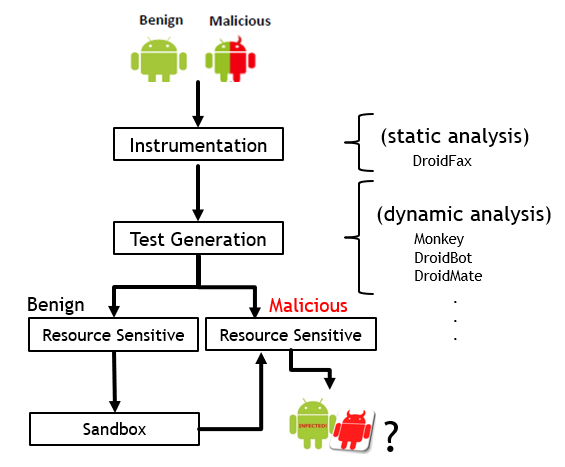
\includegraphics[width=0.45\textwidth]{images/setup.png}
%%   \label{Experiment setup}
%%   \caption{}
%%   \label{fig:setup}
%% \end{figure}

After that, we replicated the study using a configuration of DroidXP that
disables the DroidFax static analysis algorithm. With this new configuration,
we executed the benchmark one more time, using the same dataset of Android
apps, the same execution time, and the same test case generation tools.
The results of this replication allow us to compute the effective performance
of the dynamic analysis tools (RQ2)---that is, ignoring the influence of the
DroidFax static analysis algorithms.

\subsection{Second Study: Tainted analysis algorithms.}

To complement our initial study, we performed the tainted analysis at the same
data set from the first study. For this second study, we used
FlowDroid~\cite{10.1145/2666356.2594299}, a static flow analysis tool for Android apps.
The goal is to test accuracy of static analysis, through tainted analysis algorithms, at finding malicious behavior, and compare the results with previous study at the same data set.
In this second study, a behavior is considered malicious whenever the algorithms
detected a different set of source-sink pairs, coming from the benign and malign
versions of an Android app. 

Initially, Flowdroid mine all sources and sinks of each benign apps, and enumerates all possible data flows between them. Next, it performs the same process for the malicious version
of the correspondent app. In the final step, we compare the set of source-sink track between the benign app and its corresponding malicious app, in order to discovery some taint tracer different between the apps under analysis.

This study was useful to answer the third research question (RQ3), because it disclosed some pairs of applications with malicious behavior, that could not be detected at first study at none of the scenarios presented, evidencing that there is a benefit of new static analysis techniques, to complement the dynamic analysis provided by test generation tools, at mining sandboxes solutions. Details of studies results are at next section.





